\documentclass[jou]{apa6}
\usepackage[utf8]{inputenc}
\usepackage[spanish]{babel}

\usepackage{csquotes}
\usepackage[style=apa,sortcites=true,sorting=nyt,backend=biber]{biblatex}

\usepackage{listings}

\usepackage[section]{placeins}

\DeclareLanguageMapping{spanish}{spanish-apa}
\addbibresource{bibliography.bib}

\title{HPC - LAB3: Paradigma SIMT - CUDA}

\author{Rubén Cavieres Carvajal}
\affiliation{Universidad de Santiago de Chile}

\leftheader{DIINF-USACH}

\abstract{Se presenta un resumen del desarrollo del laboratorio 3 de la asignatura High Performance Computing dictado por el profesor Dr. Fernando Rannou, exponiendo resultados de las pruebas de rendimiento computacional sobre la aplicación paralelizada.}

\keywords{HPC, CUDA, NVIDIA, Parallel, Schroedinger}

\begin{document}
\maketitle
El trabajo comienza con la creación de un algoritmo secuencial que simula el comportamiento de una onda bajo la ley de Schroedinger.

Luego se identifican las piezas de código que pueden ser paralelizables para utilizar en éstas estrategias basadas en el paradigma SIMT-CUDA.

Finalmente se realizan pruebas de rendimiento de la aplicación utilizando las métricas:

\begin{itemize}
	\item Tiempo de ejecución (wall-clock) para diferentes tamaños de grillas.
	\item Ocupancia
	\item Tiempo de ejecución para diferentes tamaños de bloques.
\end{itemize}


\section{Algoritmo}
\subsection{Ecuaciones}
El algoritmo se estructuró de tal forma que represente el planteamiento del matemático. Es decir, consideró las condiciones de la variable tiempo $t$ para utilizar las ecuaciones con los siguientes métodos:

\begin{itemize}
	\item \texttt{initializeSpace}: Para $t = 0$ inicializa el espacio (grilla) de trabajo, dado por el impulso en celdas centrales en grilla.
	\item \texttt{fillSpaceFirstStep}: Para $t = 1$ genera la primera iteración de la onda utilizando $H^{t-1}$.
	\item \texttt{fillSpaceTSteps}: Para $t > 1$ genera las sucesivas iteraciones de la onda, utilizando los estados del espacio $H^{t-1}$ y $H^{t-2}$.
\end{itemize}

\subsection{Paralelización}
La estrategia de paralelización se basó en descubrir los bloques de códigos críticos potenciales para la utilización de CUDA.

Estos trozos de código fueron las ecuaciones de Schroedinger para el intervalo de tiempo $t >= 1$:

\lstset{language=C, breaklines=true, frame=single}

\begin{lstlisting}
int i = blockIdx.y * blockDim.y + threadIdx.y;
int j = blockIdx.x * blockDim.x + threadIdx.x;

waveSpace[N * i + j] = 2 * waveSpaceTMin1[N * i + j] - waveSpaceTMin2[N * i + j] + (c * c) * (dt/dd * dt/dd) * (waveSpaceTMin1[N * (i + 1) + j] + waveSpaceTMin1[N * (i - 1) + j] + waveSpaceTMin1[N * i + (j - 1)] + waveSpaceTMin1[N * i + (j + 1)] - 4 * waveSpaceTMin1[N * i + j]);
\end{lstlisting}

La estrategia adoptada fue la de utilizar las posiciones absolutas de las hebras dentro de la grilla completa, para así procesar cada porción del arreglo que contendrá imagen con expansión de onda a generar.

De esta manera, se obtienen los indices \texttt{i, j} a partir del identificador de bloque, tamaño de éste y la identificación de hebra actual.

Como se aprecia en código de instrucción \texttt{parallel for}, debido al empleo de 4 celdas que realiza la ecuación de Schroedinger, es que se decidió utilizar una paralelización estática asignando a cada hilo una cantidad fija de 4 iteraciones del bucle. 

\section{Rendimiento Computacional}

El análisis de rendimiento se realizó bajo los siguientes parámetros y tamaños:

\begin{itemize}
	\item grillas = \{512, 1024, 2048, 4096\}
	\item bloques = \{10x10, 16x16, 32x16, 32x32\}
\end{itemize}

//TODO: Hablar de bloque 10x10 para comparaciones entre dos procesadores.

Además, por problemas de capacidad de almacenamiento de equipos computacionales, debió evitarse la generación de las imágenes para cada caso.

\subsection{Tiempo (Mismo Tamaño de Bloque)}

Para los siguientes cálculos se utilizaron como tamaño de bloque \texttt{X = 10, Y = 10}:
- con generación de la imagen de salida
- sin generación de la imagen de salida.

\subsubsection{Sin Generación Imagen Salida}
El tiempo tomado para realizar la ejecución se representa en la siguiente figura:

\clearpage

\begin{figure}[h]
	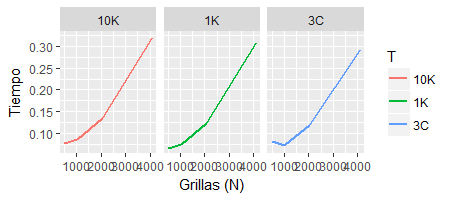
\includegraphics[width=\columnwidth]{time-same-block-size-no-raw.png}
	\caption{Tiempo ejecución para T = \{300, 1000, 10000\}}
	\label{fig:Figure1}
\end{figure}

En los tres casos el tiempo aumenta aceleradamente en una proporción similar como se evidencia en curvas. 

Sin embargo, se destaca que al aumentar el número de pasos \texttt{T}, el rendimiento del procesamiento siga siendo similar, demostrando la capacidad de la unidad GPU de procesar tareas de cómputo repetitivas. 


Se obtienen los siguientes mínimos: 

% Please add the following required packages to your document preamble:
% \usepackage{booktabs}
\begin{table}[h]
\centering
\caption{Mínimos de tiempo por iteraciones.}
\label{my-label}
\begin{tabular}{@{}lll@{}}
\toprule
\multicolumn{1}{c}{T (its.)} & \multicolumn{1}{c}{N (grilla.)} & \multicolumn{1}{c}{T (seg.)} \\ \midrule
300                          & 1024                         & 0,073585                     \\
1000                         & 512                          & 0,066303                     \\
10000                        & 512                          & 0,076833                     \\ \bottomrule
\end{tabular}
\end{table}

Como se ha dicho, estos mínimos se incrementan aceleradamente a medida que aumentan las iteraciones.

\subsubsection{Con Generación Imagen Salida}
Ejecutando algoritmo con generación de imagen, se consigue siguiente rendimiento:

\begin{figure}[h]
	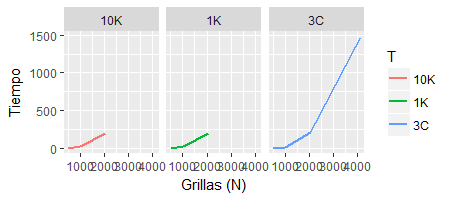
\includegraphics[width=\columnwidth]{time-same-block-size-with-raw.png}
	\caption{Tiempo ejecución para T = \{2000, 4000, 8000\}}
	\label{fig:Figure2}
\end{figure}

No fue posible continuar con resto de pruebas, debido al llenado de espacio en disco duro de computador, producto de la imagen de gran tamaño que se estaba generando para \texttt{N = 4096, T = 1000}.

El comportamiento de la curva en comparación al anterior es equivalente, registrando los siguientes mínimos:

\begin{table}[h]
\centering
\caption{Mínimos de tiempo por iteraciones.}
\label{my-label}
\begin{tabular}{@{}lll@{}}
\toprule
\multicolumn{1}{c}{T (its.)} & \multicolumn{1}{c}{N (grilla.)} & \multicolumn{1}{c}{T (seg.)} \\ \midrule
300                          & 512                          & 0.244316                     \\
1000                         & 512                          & 0.284443                     \\
10000                        & 512                          & 0.296664                     \\ \bottomrule
\end{tabular}
\end{table}

Los tiempos mínimos no experimentan mayores cambios, en comparación con los máximos:

// TODO: completar con info.
\begin{table}[h]
	\centering
	\caption{Máximos de tiempo por iteraciones.}
	\label{my-label}
	\begin{tabular}{@{}lll@{}}
		\toprule
		\multicolumn{1}{c}{T (its.)} & \multicolumn{1}{c}{N (grilla.)} & \multicolumn{1}{c}{T (seg.)} \\ \midrule
		300                          & 512                          & 0.244316                     \\
		1000                         & 512                          & 0.284443                     \\
		10000                        & 512                          & 0.296664                     \\ \bottomrule
	\end{tabular}
\end{table}

Dichos tiempos fueron excesivamente altos, evidenciando el costo computacional que implica el acceso a memoria secundaria, por ser aquella más lenta dentro de todos los tipos de memoria del sistema.

\FloatBarrier

\subsection{Ocupancia}
La métrica utilizada para calcular el \textit{Device Occupancy} se expresa de la siguiente forma:

\[
	Ocupancia = \frac{Numero\, de\, warps\, activos}{Maximo\, Numero\, de\, warps}
\]

// TODO: calcularlo.

\subsection{Tiempo (Diferentes Tamaños de Bloques, Sin Imagen Salida)}
Para este caso se utilizaron los parámetros:

\begin{itemize}
	\item grilla = \{2048x2048\}
	\item bloques = \{16x16, 32x16, 32x32\}
\end{itemize}

Curva generada fue la siguiente:

// TODO: hacer curva
\begin{figure}[h]
	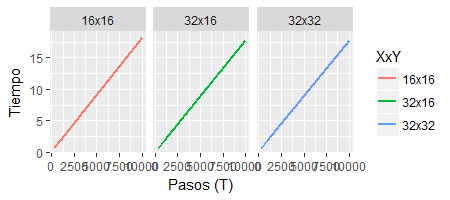
\includegraphics[width=\columnwidth]{time-diff-block-size-no-raw.png}
	\caption{Eficiencia para T = \{2000, 4000, 8000\}}
	\label{fig:Figure3}
\end{figure}

// TODO: Describir y tabla.
Hay un decremento sostenido del indicador hasta la ejecución con 3 hebras, desde donde curva se estabiliza.

El punto de inflexión dado con \textit{H = 3} para cada iteración tiene el siguiente valor:

\begin{table}[]
\centering
\caption{Punto inflexión eficiencia por iteraciones}
\label{my-label}
\begin{tabular}{@{}lll@{}}
\toprule
\multicolumn{1}{c}{T (its.)} & \multicolumn{1}{c}{H (num.)} & \multicolumn{1}{c}{E(H)} \\ \midrule
2000                         & 3                            & 0,3718947                \\
4000                         & 3                            & 0,3491872                \\
8000                         & 3                            & 0,352224                 \\ \bottomrule
\end{tabular}
\end{table}

\section{Conclusiones}
// TODO: hacerlas

A partir de la comparación de los resultados para cada variación de parámetro del algoritmo, se observa que las curvas de tiempo, \textit{speedup} y eficiencia se presentan similares, evidenciando que la estrategia de paralelización aplicada fue estática. 

Esta característica de paralelización garantizó que el trabajo con hilos se realizara uniformemente dentro del bucle de construcción de grilla con imagen.

Un inconveniente en el análisis de rendimiento fue que se contó con un computador de 8 núcleos, cuya característica no permitió extender el análisis con una mayor cantidad de cómputo que permitiera ver el comportamiento de la aplicación en un periodo de tiempo más extenso.

\end{document}
